\documentclass[12pt,a4paper]{report}

% ── pachete de baza ──────────────────────────────────────────────────────────
\usepackage[utf8]{inputenc}
\usepackage[T1]{fontenc}
\usepackage[romanian]{babel}
\usepackage{geometry}
\geometry{margin=2.5cm}

% ── tipografie ────────────────────────────────────────────────────────────────
\usepackage{lmodern}
\usepackage{microtype}
\usepackage{setspace}
\onehalfspacing

% ── titlu si sectiuni ─────────────────────────────────────────────────────────
\usepackage{titlesec}
\titleformat{\chapter}[block]{\Large\bfseries}{Capitolul \thechapter.}{0.5em}{}
\titleformat{\section}{\large\bfseries}{\thesection}{0.5em}{}
\titleformat{\subsection}{\normalsize\bfseries}{\thesubsection}{0.5em}{}

% ── cuprins ───────────────────────────────────────────────────────────────────
\usepackage{tocloft}
\setlength{\cftsecindent}{1.5em}

% ── grafice si imagini ────────────────────────────────────────────────────────
\usepackage{graphicx}
\usepackage{float}
\usepackage[labelfont=bf, font=small]{caption}
\graphicspath{{figures/}}

% ── cod sursa ─────────────────────────────────────────────────────────────────
\usepackage{listings}
\usepackage{xcolor}

\definecolor{codebg}{RGB}{245,245,245}
\definecolor{codeframe}{RGB}{200,200,200}
\definecolor{kwcolor}{RGB}{0,0,180}
\definecolor{strcolor}{RGB}{180,0,0}
\definecolor{cmtcolor}{RGB}{80,120,80}
\definecolor{numcolor}{RGB}{100,0,150}

\lstdefinestyle{python}{
    language=Python,
    backgroundcolor=\color{codebg},
    frame=single,
    rulecolor=\color{codeframe},
    basicstyle=\ttfamily\small,
    keywordstyle=\color{kwcolor}\bfseries,
    stringstyle=\color{strcolor},
    commentstyle=\color{cmtcolor}\itshape,
    numberstyle=\tiny\color{numcolor},
    numbers=left,
    numbersep=8pt,
    showstringspaces=false,
    breaklines=true,
    breakatwhitespace=true,
    tabsize=4,
    captionpos=b,
    morekeywords={self, True, False, None},
}

\lstdefinestyle{yaml}{
    language={},
    backgroundcolor=\color{codebg},
    frame=single,
    rulecolor=\color{codeframe},
    basicstyle=\ttfamily\small,
    keywordstyle=\color{kwcolor}\bfseries,
    stringstyle=\color{strcolor},
    commentstyle=\color{cmtcolor}\itshape,
    numbers=left,
    numberstyle=\tiny\color{numcolor},
    numbersep=8pt,
    showstringspaces=false,
    breaklines=true,
    tabsize=2,
    captionpos=b,
    morecomment=[l]{\#},
    morestring=[b]",
    morestring=[b]',
}

% ── tabele ────────────────────────────────────────────────────────────────────
\usepackage{booktabs}
\usepackage{tabularx}
\usepackage{array}

% ── referinte si linkuri ──────────────────────────────────────────────────────
\usepackage[hidelinks]{hyperref}

% ── diagrame / tikz ───────────────────────────────────────────────────────────
\usepackage{tikz}
\usetikzlibrary{shapes.geometric, arrows.meta, positioning, fit, backgrounds}

% ── utilitare ─────────────────────────────────────────────────────────────────
\usepackage{enumitem}
\usepackage{amsmath}
\usepackage{amssymb}

% ═════════════════════════════════════════════════════════════════════════════
\begin{document}

% ── pagina de titlu ──────────────────────────────────────────────────────────
\begin{titlepage}
\centering
\vspace*{2cm}
{\Huge\bfseries Sistem de Recomandare Muzicală\\Bazat pe Inteligență Artificială\par}
\vspace{0.5cm}
{\large Arhitectură Multi-Agent cu CrewAI, SHAP și XGBoost\par}
\vspace{2cm}
\includegraphics[width=0.25\textwidth]{figures/logo_placeholder.png}
\vspace{2cm}

{\large\itshape Documentație Tehnică\par}
\vfill
{\large 2025\par}
\end{titlepage}

\tableofcontents
\newpage

% ═══════════════════════════════════════════════════════════════════════════
\chapter{Introducere și Ideea Principală}
% ═══════════════════════════════════════════════════════════════════════════

\section{Motivație}

Sistemele de recomandare muzicală existente (Spotify Discover Weekly, Last.fm)
funcționează cu algoritmi de filtrare colaborativă sau bazați pe istoricul de
ascultare al utilizatorilor. Aceștia nu explică de ce o piesă a fost
recomandată și nu sunt transparenți în privința caracteristicilor audio care
stau la baza recomandării.

Proiectul de față propune un sistem alternativ care:
\begin{itemize}[noitemsep]
    \item identifică caracteristicile sonore ale unei piese de intrare din date reale Spotify;
    \item caută piesele cel mai similare din punct de vedere audio;
    \item explică \textit{de ce} fiecare piesă a fost recomandată, folosind valori SHAP
          derivate dintr-un clasificator XGBoost antrenat pe gen muzical;
    \item prezintă rezultatele printr-o interfață de tip terminal cu agenți AI care
          colaborează autonom.
\end{itemize}

\section{Ideea de Bază}

Dat un titlu de piesă și un artist, sistemul parcurge trei etape principale:

\begin{enumerate}
    \item \textbf{Analiză sonoră} — extragerea celor 9 caracteristici audio Spotify
          (danceability, energy, loudness etc.) din dataset.
    \item \textbf{Căutare de piese similare} — identificarea genului muzical prin
          amprente sonore și găsirea celor mai apropiate 5 piese prin similaritate cosinus.
    \item \textbf{Explicabilitate} — calculul valorilor SHAP pentru fiecare recomandare,
          cuantificând contribuția fiecărei caracteristici audio la predicția de gen.
\end{enumerate}

Întreaga logică este orchestrată de trei agenți AI autonomi care rulează
secvențial în cadrul framework-ului \textit{CrewAI}.

\begin{figure}[H]
\centering
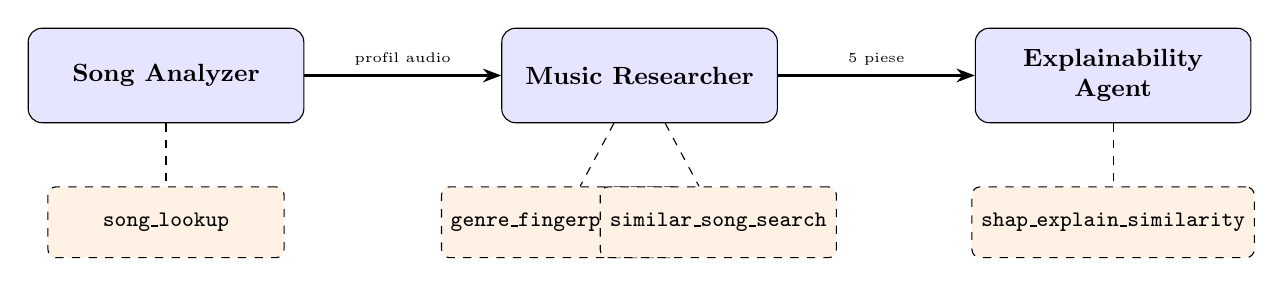
\begin{tikzpicture}[
    agent/.style={draw, rounded corners=5pt, fill=blue!10, minimum width=3.5cm,
                  minimum height=1.2cm, align=center, font=\small\bfseries},
    tool/.style={draw, dashed, rounded corners=3pt, fill=orange!10, minimum width=3cm,
                 minimum height=0.9cm, align=center, font=\footnotesize},
    arrow/.style={-Stealth, thick},
    node distance=1.5cm and 2.5cm
]
\node[agent] (a1) {Song Analyzer};
\node[agent, right=of a1] (a2) {Music Researcher};
\node[agent, right=of a2] (a3) {Explainability\\Agent};

\node[tool, below=0.8cm of a1] (t1) {\texttt{song\_lookup}};
\node[tool, below=0.8cm of a2, xshift=-1cm] (t2) {\texttt{genre\_fingerprinter}};
\node[tool, below=0.8cm of a2, xshift=1cm] (t3) {\texttt{similar\_song\_search}};
\node[tool, below=0.8cm of a3] (t4) {\texttt{shap\_explain\_similarity}};

\draw[arrow] (a1) -- (a2) node[midway, above, font=\tiny] {profil audio};
\draw[arrow] (a2) -- (a3) node[midway, above, font=\tiny] {5 piese};
\draw[dashed] (a1) -- (t1);
\draw[dashed] (a2) -- (t2);
\draw[dashed] (a2) -- (t3);
\draw[dashed] (a3) -- (t4);
\end{tikzpicture}
\caption{Fluxul de procesare al sistemului multi-agent}
\label{fig:flux}
\end{figure}

% ═══════════════════════════════════════════════════════════════════════════
\chapter{Stack Tehnologic}
% ═══════════════════════════════════════════════════════════════════════════

\begin{table}[H]
\centering
\renewcommand{\arraystretch}{1.3}
\begin{tabularx}{\textwidth}{@{}llX@{}}
\toprule
\textbf{Componentă} & \textbf{Versiune} & \textbf{Rol} \\
\midrule
Python          & $\geq$3.10   & Limbajul de implementare principal \\
CrewAI          & $\geq$0.102  & Orchestrare agenți AI (framework multi-agent) \\
Ollama / LLaMA 3.2 & local     & LLM-ul folosit de fiecare agent pentru raționament \\
XGBoost         & $\geq$3.2    & Clasificator de gen muzical (11 trăsături, 17 clase) \\
SHAP            & $\geq$0.49   & Explicabilitate prin valori Shapley pentru XGBoost \\
scikit-learn    & $\geq$1.7    & LabelEncoder, train/test split, cross-validare \\
pandas          & $\geq$2.0    & Manipularea și filtrarea datasetului \\
NumPy           & $\geq$1.26   & Calcule vectoriale, similaritate cosinus \\
Kaggle API      & $\geq$1.7    & Descărcare automată a dataseturilor Kaggle \\
uv              & —            & Manager de dependențe și lansare aplicație \\
\bottomrule
\end{tabularx}
\caption{Stack-ul tehnologic al proiectului}
\label{tab:techstack}
\end{table}

\section{Modelul de Limbaj}

Sistemul utilizează \textbf{LLaMA 3.2} rulat local prin \textbf{Ollama},
configurabil din fișierul \texttt{.env}:

\begin{lstlisting}[style=yaml, caption={Configurare model LLM (.env)}]
MODEL=ollama/llama3.2
OPENAI_API_KEY=ollama
\end{lstlisting}

Alegerea unui LLM local elimină costurile API și menține datele private, dar
implică un plafon de calitate al răspunsurilor mai scăzut decât modelele cloud
(GPT-4, Claude 3). Totuși, logica de calcul (SHAP, cosinus, XGBoost) este
determinista și independenta de LLM — acesta serveste doar ca motor de
raționament și sinteză textuală.

% ═══════════════════════════════════════════════════════════════════════════
\chapter{Datasetul Utilizat}
% ═══════════════════════════════════════════════════════════════════════════

\section{Sursele de Date}

Sistemul combină două surse principale de date, obținând un dataset final de
recomandare cu mii de piese etichetate cu gen muzical și caracteristici audio.

\subsection{Sursa Zenodo}

Fișierul \texttt{zenodo.csv} conține date extrase direct din API-ul Spotify,
cu câmpuri standardizate. Este sursa \textbf{primară}: la deduplicare, rândul
Zenodo câștigă față de cel Kaggle.

\subsection{Sursele Kaggle}

Șapte fișiere CSV descărcate de pe Kaggle, fiecare cu scheme diferite:

\begin{table}[H]
\centering
\renewcommand{\arraystretch}{1.2}
\begin{tabularx}{\textwidth}{@{}lX@{}}
\toprule
\textbf{Fișier} & \textbf{Particularități} \\
\midrule
\texttt{dataset.csv}             & Schema standard Spotify \\
\texttt{train.csv}               & Schema standard, similar cu dataset.csv \\
\texttt{ClassicHit.csv}          & Coloane cu majuscule, key ca notă muzicală \\
\texttt{Music Info.csv}          & Genre extras din câmpul \texttt{tags} când lipsește \\
\texttt{SpotifyFeatures.csv}     & Key ca notă (C, C\#…), mode ca Major/Minor \\
\texttt{top\_10000\_1950-now.csv} & Trăsăturile ca string cu ghilimele \\
\texttt{top\_10000\_1960-now.csv} & Identic cu cel de mai sus \\
\bottomrule
\end{tabularx}
\caption{Fișierele CSV Kaggle utilizate}
\end{table}

\section{Caracteristicile Audio}

Fiecare piesă este descrisă prin 9 caracteristici numerice Spotify și 2
caracteristici suplimentare utilizate de clasificatorul XGBoost:

\begin{table}[H]
\centering
\renewcommand{\arraystretch}{1.2}
\begin{tabularx}{\textwidth}{@{}llX@{}}
\toprule
\textbf{Caracteristică} & \textbf{Interval} & \textbf{Semnificație} \\
\midrule
\texttt{danceability}     & 0–1    & Potrivirea pentru dans (ritm, tempo, regularitate) \\
\texttt{energy}           & 0–1    & Intensitate percepută (viteză, volum, timbru) \\
\texttt{loudness}         & $-$60–0 dB & Volumul mediu al piesei \\
\texttt{speechiness}      & 0–1    & Prezența vorbirii în piesă \\
\texttt{acousticness}     & 0–1    & Probabilitatea că piesa este acustică \\
\texttt{instrumentalness} & 0–1    & Absența vocalelor (1 = pur instrumental) \\
\texttt{liveness}         & 0–1    & Probabilitatea că e o înregistrare live \\
\texttt{valence}          & 0–1    & Pozitivitate muzicală (0 = trist, 1 = fericit) \\
\texttt{tempo}            & BPM    & Ritmul estimat în bătăi pe minut \\
\midrule
\texttt{key}              & 0–11   & Tonalitatea piesei (0=C, 1=C\#, …, 11=B) \\
\texttt{mode}             & 0/1    & Mod Major (1) sau Minor (0) \\
\bottomrule
\end{tabularx}
\caption{Caracteristicile audio ale fiecărei piese}
\label{tab:features}
\end{table}

\section{Amprentele de Gen}

Pe lângă dataset, sistemul folosește un fișier de amprente sonore
(\texttt{data/genre\_fingerprints}) care definește 30 de profiluri de gen, fiecare
cu valorile tipice ale celor 9 caracteristici și semnalele cheie care îl
caracterizează. Exemplu:

\begin{lstlisting}[style=yaml, caption={Fragment din fișierul genre\_fingerprints}]
## Metal
danceability: 0.32
energy: 0.91
loudness: 87.0
speechiness: 0.06
acousticness: 0.04
instrumentalness: 0.20
liveness: 0.14
valence: 0.22
tempo: 62.0
key signals: extreme energy+loudness, very low valence, low danceability
\end{lstlisting}

Fiecare gen este reprezentat ca un vector în spațiul celor 9 caracteristici,
permițând clasificarea prin \textbf{similaritate cosinus față de centroid}.

% ═══════════════════════════════════════════════════════════════════════════
\chapter{Scripturile de Procesare a Datelor}
% ═══════════════════════════════════════════════════════════════════════════

Cele patru scripturi din directorul \texttt{scripts/} trebuie rulate în ordine,
o singură dată, pentru a construi datasetul final și a antrena clasificatorul.

\begin{figure}[H]
\centering
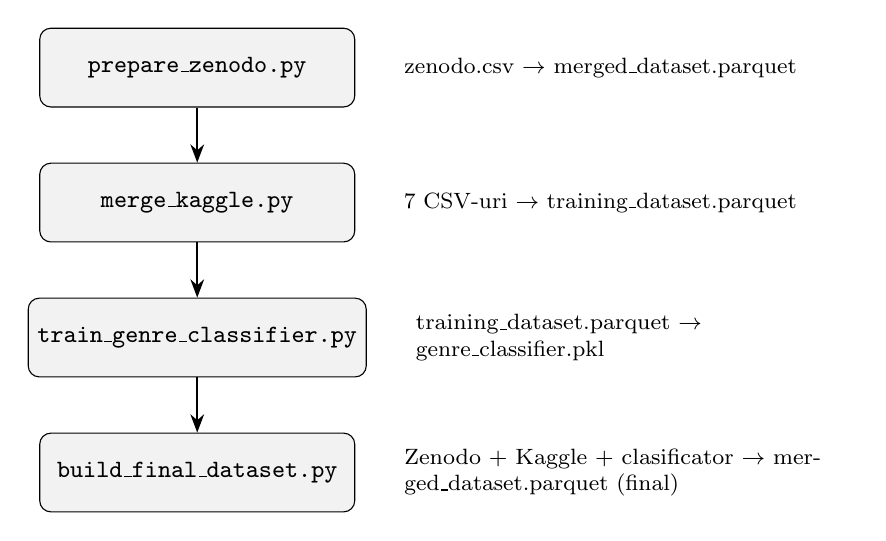
\begin{tikzpicture}[
    box/.style={draw, rounded corners=4pt, fill=gray!10, minimum width=4cm,
                minimum height=1cm, align=center, font=\small\ttfamily},
    arrow/.style={-Stealth, thick},
    node distance=0.7cm
]
\node[box] (s1) {prepare\_zenodo.py};
\node[box, below=of s1] (s2) {merge\_kaggle.py};
\node[box, below=of s2] (s3) {train\_genre\_classifier.py};
\node[box, below=of s3] (s4) {build\_final\_dataset.py};

\draw[arrow] (s1) -- (s2);
\draw[arrow] (s2) -- (s3);
\draw[arrow] (s3) -- (s4);

\node[right=0.5cm of s1, font=\footnotesize, text width=5.5cm]
    {zenodo.csv $\to$ merged\_dataset.parquet};
\node[right=0.5cm of s2, font=\footnotesize, text width=5.5cm]
    {7 CSV-uri $\to$ training\_dataset.parquet};
\node[right=0.5cm of s3, font=\footnotesize, text width=5.5cm]
    {training\_dataset.parquet $\to$ genre\_classifier.pkl};
\node[right=0.5cm of s4, font=\footnotesize, text width=5.5cm]
    {Zenodo + Kaggle + clasificator $\to$ merged\_dataset.parquet (final)};
\end{tikzpicture}
\caption{Lanțul de procesare a datelor}
\label{fig:pipeline}
\end{figure}

\section{prepare\_zenodo.py}

Convertește \texttt{zenodo.csv} în format Parquet, normalizând coloanele și
extragând primul gen dintr-o lista stringificată de genuri.

\begin{lstlisting}[style=python, caption={Extragerea primului gen din lista Zenodo}]
def _parse_first_genre(raw) -> str:
    if not isinstance(raw, str):
        return "unknown"
    raw = raw.strip()
    if raw in ("[]", "nan", ""):
        return "unknown"
    try:
        parsed = ast.literal_eval(raw)
        if isinstance(parsed, list) and parsed:
            return str(parsed[0]).strip()
    except (ValueError, SyntaxError):
        pass
    cleaned = raw.strip("[]").replace("'", "").replace('"', "").split(",")
    first = cleaned[0].strip()
    return first if first else "unknown"
\end{lstlisting}

Deduplicarea se face după cheia \texttt{(track\_name, artists)}, păstrând
rândul cu cel mai mare scor de popularitate și cu gen cunoscut.

\section{merge\_kaggle.py}

Combină cele 7 fișiere CSV Kaggle într-un singur \texttt{training\_dataset.parquet}.
Fiecare fișier are un loader dedicat care normalizează coloanele la schema standard.

\begin{lstlisting}[style=python, caption={Loader pentru ClassicHit.csv (coloane cu majuscule)}]
def load_classichit() -> pd.DataFrame:
    df = pd.read_csv(_p("ClassicHit.csv"), low_memory=False)
    df = df.rename(columns={
        "Track": "track_name",
        "Artist": "artists",
        "Genre": "track_genre"
    })
    feat_rename = {
        "Danceability": "danceability", "Energy": "energy",
        "Loudness": "loudness", "Speechiness": "speechiness",
        "Acousticness": "acousticness", "Instrumentalness": "instrumentalness",
        "Liveness": "liveness", "Valence": "valence", "Tempo": "tempo",
    }
    df = df.rename(columns=feat_rename)
    return _finalize(df, "ClassicHit")
\end{lstlisting}

Genurile care nu aparțin unui sistem de recomandare muzicală (comedy, anime,
soundtrack, opera, movie) sunt eliminate. Deduplicarea prioritizează rândul cu
gen cunoscut și cu popularitate maximă.

\section{train\_genre\_classifier.py}

Antrenează clasificatorul XGBoost pe \texttt{training\_dataset.parquet} cu
validare încrucișată stratificată pe 5 folduri.

\begin{lstlisting}[style=python, caption={Antrenarea clasificatorului XGBoost cu cross-validare}]
model_cv = xgb.XGBClassifier(
    n_estimators=200,
    max_depth=7,
    learning_rate=0.1,
    subsample=0.8,
    colsample_bytree=0.8,
    tree_method="hist",
    eval_metric="mlogloss",
    random_state=42,
)
skf = StratifiedKFold(n_splits=5, shuffle=True, random_state=42)
cv_scores = cross_val_score(model_cv, X, y, cv=skf,
                            scoring="accuracy", n_jobs=-1)
print(f"Mean accuracy: {cv_scores.mean():.3f} (+/- {cv_scores.std():.3f})")
\end{lstlisting}

Clasele cu mai puțin de 100 de exemple sunt eliminate. Valoarea $-1$ pentru
\texttt{key} și \texttt{mode} (necunoscute) este înlocuită cu \texttt{NaN},
gestionat nativ de XGBoost.

\section{build\_final\_dataset.py}

Combina datasetul Zenodo cu cel Kaggle. Piesele din Zenodo al căror gen
consolidat nu se regăsește în cele 17 clase ale clasificatorului primesc o
predicție XGBoost. Zenodo este prioritar la deduplicare.

\begin{lstlisting}[style=python, caption={Predicție XGBoost pentru piese fără gen în Zenodo}]
df_zenodo["track_genre"] = df_zenodo["track_genre"].apply(_consolidate_genre)
needs_pred = ~df_zenodo["track_genre"].isin(trained_classes)

if needs_pred.any():
    df_zenodo.loc[needs_pred, "track_genre"] = _predict_genres(
        df_zenodo[needs_pred], model, le
    )
\end{lstlisting}

\section{Consolidarea Genurilor}

Funcția \texttt{\_consolidate\_genre()} mapează sute de sub-genuri Spotify la
17 clase largi folosite de clasificator, prin expresii regulate ordonate cu
prioritate:

\begin{lstlisting}[style=python, caption={Fragment din \_consolidate\_genre() — prioritate metal > rock}]
# metal inainte de rock pentru a evita suprapunerile
if re.search(r"death.metal|black.metal|power.metal|thrash.metal|"
             r"heavy.metal|doom.metal|metalcore|nu.metal", g):
    return "metal"
if re.search(r"\bmetal\b", g):
    return "metal"

# subgenuri de rock
if re.search(r"grunge|prog.*rock|classic.rock|hard.rock|"
             r"brit.pop|shoegaze|alt.rock", g):
    return "rock"
if re.search(r"\brock\b", g):
    return "rock"
\end{lstlisting}

Cele 17 clase finale sunt: \textit{ambient, blues, classical, country,
electronic, folk, hip-hop, jazz, k-pop, latin, metal, pop, r\&b, reggae,
rock, ska, world}.

% ═══════════════════════════════════════════════════════════════════════════
\chapter{Arhitectura Sistemului Multi-Agent}
% ═══════════════════════════════════════════════════════════════════════════

\section{Framework-ul CrewAI}

CrewAI este un framework Python pentru orchestrarea agenților AI care
colaborează pentru a rezolva sarcini complexe. Fiecare agent are:
\begin{itemize}[noitemsep]
    \item un \textbf{rol} și un \textbf{scop} definite în \texttt{agents.yaml};
    \item un set de \textbf{instrumente} (tools) pe care le poate apela;
    \item un \textbf{LLM} pentru raționament (LLaMA 3.2 prin Ollama).
\end{itemize}

Crew-ul este configurat cu \textbf{procesare secvențială}: fiecare agent
primește rezultatele agentului precedent prin mecanismul de \texttt{context}.

\begin{lstlisting}[style=python, caption={Definirea crew-ului în crew.py}]
@crew
def crew(self) -> Crew:
    return Crew(
        agents=self.agents,
        tasks=self.tasks,
        process=Process.sequential,
        verbose=True,
    )
\end{lstlisting}

\section{Fluxul ReAct}

Fiecare agent urmează ciclul \textbf{ReAct} (Reason + Act):
\begin{enumerate}[noitemsep]
    \item \textit{Thought} — agentul decide ce acțiune să facă;
    \item \textit{Action} — apelează un tool cu parametrii corecți;
    \item \textit{Observation} — primește rezultatul tool-ului;
    \item Repetă până când poate formula un \textit{Final Answer}.
\end{enumerate}

\begin{figure}[H]
\centering
\includegraphics[width=0.9\textwidth]{figures/screenshot_react_flow.png}
\caption{Exemplu de ciclu ReAct în terminal (Thought / Action / Observation)}
\label{fig:react}
\end{figure}

% ═══════════════════════════════════════════════════════════════════════════
\chapter{Agenții}
% ═══════════════════════════════════════════════════════════════════════════

\section{Song Analyzer}

\begin{table}[H]
\renewcommand{\arraystretch}{1.2}
\begin{tabularx}{\textwidth}{@{}lX@{}}
\toprule
\textbf{Câmp} & \textbf{Valoare} \\
\midrule
Rol      & Music Characteristics Analyst \\
Tool     & \texttt{song\_lookup} \\
Scop     & Extragerea celor 9 caracteristici audio ale piesei de intrare \\
Context  & — (primul agent) \\
\bottomrule
\end{tabularx}
\caption{Configurarea agentului Song Analyzer}
\end{table}

Agentul apelează \texttt{song\_lookup} cu titlul și artistul, extrage valorile
numerice din rezultat și produce un profil muzical structurat cu interpretare
în limbaj natural (de ex. \textit{``energy=0.87 → piesă intensă, rapidă, puternică''}).

\begin{lstlisting}[style=yaml, caption={Configurarea agentului song\_analyzer în agents.yaml}]
song_analyzer:
  llm: ollama/llama3.2
  role: Music Characteristics Analyst
  goal: >
    Look up "{song_title}" by "{artist}" in the dataset using the song_lookup
    tool and produce a detailed musical profile covering all 9 audio features,
    genre, popularity, and a plain-language interpretation of each feature.
  backstory: >
    You are an expert musicologist with deep knowledge of Spotify audio feature
    analysis. You extract precise numerical characteristics from songs and
    translate them into meaningful musical descriptions.
\end{lstlisting}

\begin{figure}[H]
\centering
\includegraphics[width=0.9\textwidth]{figures/screenshot_agent1_output.png}
\caption{Outputul agentului Song Analyzer — profilul audio al piesei de intrare}
\label{fig:agent1}
\end{figure}

\section{Music Researcher}

\begin{table}[H]
\renewcommand{\arraystretch}{1.2}
\begin{tabularx}{\textwidth}{@{}lX@{}}
\toprule
\textbf{Câmp} & \textbf{Valoare} \\
\midrule
Rol      & Genre-Aware Music Similarity Researcher \\
Tools    & \texttt{genre\_fingerprinter}, \texttt{similar\_song\_search} \\
Scop     & Identificarea genului și găsirea celor mai similare 5 piese \\
Context  & Rezultatele lui Song Analyzer \\
\bottomrule
\end{tabularx}
\caption{Configurarea agentului Music Researcher}
\end{table}

Agentul urmează doi pași:
\begin{enumerate}
    \item \textbf{Amprentă de gen} — apelează \texttt{genre\_fingerprinter} și
          identifică genul dominant (top 1 din 30 de amprente) prin similari-
          tate cosinus pe vectorul celor 9 caracteristici scalate.
    \item \textbf{Căutare similară} — apelează \texttt{similar\_song\_search}
          cu filtru implicit pe genul detectat, returnând 5 piese ordonate după
          scorul de similaritate cosinus pe caracteristici normalizate.
\end{enumerate}

\begin{figure}[H]
\centering
\includegraphics[width=0.9\textwidth]{figures/screenshot_agent2_output.png}
\caption{Outputul agentului Music Researcher — amprenta de gen și top 5 piese similare}
\label{fig:agent2}
\end{figure}

\section{Explainability Agent}

\begin{table}[H]
\renewcommand{\arraystretch}{1.2}
\begin{tabularx}{\textwidth}{@{}lX@{}}
\toprule
\textbf{Câmp} & \textbf{Valoare} \\
\midrule
Rol      & SHAP and Fingerprint Music Recommendation Specialist \\
Tool     & \texttt{shap\_explain\_similarity} \\
Scop     & Explicarea fiecărei recomandări prin valori SHAP \\
Context  & Rezultatele lui Music Researcher \\
Output   & Raport Markdown salvat în \texttt{output/recommendations.md} \\
\bottomrule
\end{tabularx}
\caption{Configurarea agentului Explainability Agent}
\end{table}

Agentul apelează \texttt{shap\_explain\_similarity} pentru fiecare din cele 5
piese recomandate, combina scorurile SHAP cu semnalele de amprentă și redactează
un paragraf explicativ pentru fiecare recomandare în limbaj natural.

\begin{figure}[H]
\centering
\includegraphics[width=0.9\textwidth]{figures/screenshot_agent3_output.png}
\caption{Outputul agentului Explainability Agent — raport final de recomandări}
\label{fig:agent3}
\end{figure}

% ═══════════════════════════════════════════════════════════════════════════
\chapter{Task-urile}
% ═══════════════════════════════════════════════════════════════════════════

Cele trei task-uri sunt definite în \texttt{config/tasks.yaml} și sunt
executate secvențial.

\section{analyze\_song\_task}

\begin{lstlisting}[style=yaml, caption={Definiția task-ului analyze\_song\_task}]
analyze_song_task:
  description: >
    Use the song_lookup tool to find "{song_title}" by "{artist}" in the dataset.
    Produce a structured musical profile with:
    1. Exact values for all 9 audio features
    2. The song's dataset genre and popularity score
    3. A plain-language interpretation of each key feature
    4. A one-paragraph summary of what makes this song sonically distinctive
  expected_output: >
    A structured musical profile with all 9 numerical audio features,
    plain-language interpretations, and a summary paragraph.
  agent: song_analyzer
\end{lstlisting}

\section{research\_similar\_songs\_task}

\begin{lstlisting}[style=yaml, caption={Definiția task-ului research\_similar\_songs\_task}]
research_similar_songs_task:
  description: >
    STEP 1 - Genre Fingerprinting:
    Call genre_fingerprinter with song_title and artist.
    Record top 3 genre matches with similarity scores and key signals.

    STEP 2 - Similar Song Search:
    Call similar_song_search with song_title, artist and top_n=5.
    Record each result: track_name, artists, genre, popularity, similarity_score.
  expected_output: >
    Part 1 - Genre fingerprint analysis with predicted genre and key signals.
    Part 2 - Ranked list of 5 similar songs with similarity scores.
  agent: music_researcher
  context:
    - analyze_song_task
\end{lstlisting}

\section{explain\_and\_recommend\_task}

\begin{lstlisting}[style=yaml, caption={Definiția task-ului explain\_and\_recommend\_task}]
explain_and_recommend_task:
  description: >
    Call shap_explain_similarity for each of the 5 similar songs.
    After all calls, write a Markdown report in plain English.

    IMPORTANT: Do NOT copy or output any JSON or raw tool data.
    Write only human-readable text.

    Report format:
    ## Music Recommendations for {song_title} by {artist}
    One intro sentence about the input song's genre and sound.
    ### 1. Track Name - Artist
    Genre: <genre> | Similarity: <fingerprint_cosine_similarity>
    <One paragraph: why this song is similar...>
  expected_output: >
    A Markdown report with 5 numbered entries, each with a plain-English
    paragraph explaining the recommendation based on shared audio features.
  agent: explainability_agent
  context:
    - research_similar_songs_task
  output_file: output/recommendations.md
  markdown: true
\end{lstlisting}

% ═══════════════════════════════════════════════════════════════════════════
\chapter{Instrumentele (Tools)}
% ═══════════════════════════════════════════════════════════════════════════

Toate instrumentele moștenesc din \texttt{crewai.tools.BaseTool} și definesc
schema de input cu \texttt{pydantic}.

\section{SongLookupTool}

\textbf{Nume:} \texttt{song\_lookup} \quad
\textbf{Fișier:} \texttt{tools/dataset\_tools.py}

Caută o piesă în dataset după titlu și artist, returnând caracteristicile audio
ca JSON. Căutarea este case-insensitive și tolerantă la potriviri parțiale;
în caz de nepotrivire returnează sugestii bazate pe primele 5 caractere ale titlului.

\begin{lstlisting}[style=python, caption={Logica de căutare din SongLookupTool}]
def _find_index(df, song_title, artist=""):
    title_lower = song_title.lower()
    title_mask = df["track_name"].str.lower().str.contains(
        title_lower, na=False, regex=False
    )
    if artist:
        artist_mask = df["artists"].str.lower().str.contains(
            artist.lower(), na=False, regex=False
        )
        combined = title_mask & artist_mask
        mask = combined if combined.any() else title_mask
    else:
        mask = title_mask

    hits = df[mask]
    if hits.empty:
        return None
    exact = hits[hits["track_name"].str.lower() == title_lower]
    source = exact if not exact.empty else hits
    return int(source["popularity"].idxmax())
\end{lstlisting}

\textbf{Output exemplu:}
\begin{lstlisting}[style=yaml]
{
  "track_name": "Bohemian Rhapsody",
  "artists": "Queen",
  "genre": "rock",
  "popularity": 88,
  "features": {
    "danceability": 0.3963, "energy": 0.4004,
    "loudness": -11.1, "valence": 0.2406, "tempo": 71.066
  }
}
\end{lstlisting}

\section{GenreFingerprinterTool}

\textbf{Nume:} \texttt{genre\_fingerprinter} \quad
\textbf{Fișier:} \texttt{tools/dataset\_tools.py}

Identifică genul muzical al unei piese prin similaritate cosinus față de 30 de
amprente de gen predefinite. Vectorul piesei este scalat la intervalul 0–100
(similar scalei amprentelor) înainte de calcul.

\begin{lstlisting}[style=python, caption={Scalarea la scara amprentei și calculul cosinus}]
def _to_fingerprint_scale(row) -> np.ndarray:
    vec = []
    for feat in NUMERIC_FEATURES:
        val = float(row[feat])
        if feat == "loudness":
            scaled = (val + 60.0) / 60.0 * 100.0
        elif feat == "tempo":
            scaled = val / 220.0 * 100.0
        else:
            scaled = val * 100.0
        vec.append(max(0.0, min(100.0, scaled)))
    return np.array(vec)

# calcul similaritate cosinus pentru fiecare amprenta
song_vec = _to_fingerprint_scale(row)
song_norm = np.linalg.norm(song_vec) or 1.0
for fp in fps.values():
    fp_norm = np.linalg.norm(fp["vector"]) or 1.0
    sim = float(np.dot(song_vec, fp["vector"]) / (song_norm * fp_norm))
\end{lstlisting}

Returnează top 3 genuri cu scoruri și o comparație caracteristică cu amprenta
câștigătoare (delta față de valorile așteptate).

\section{SimilarSongSearchTool}

\textbf{Nume:} \texttt{similar\_song\_search} \quad
\textbf{Fișier:} \texttt{tools/dataset\_tools.py}

Găsește cele mai similare $N$ piese față de piesa de referință prin
\textbf{similaritate cosinus pe caracteristici normalizate min-max}.

\begin{align}
\text{sim}(u, v) = \frac{u \cdot v}{\|u\| \cdot \|v\|}
\end{align}

\begin{lstlisting}[style=python, caption={Căutarea vectorizată a pieselor similare}]
ref_vec = norm[ref_idx]
ref_norm = np.linalg.norm(ref_vec) or 1.0
row_norms = np.linalg.norm(norm, axis=1)
row_norms = np.where(row_norms == 0, 1.0, row_norms)
similarities = (norm @ ref_vec) / (row_norms * ref_norm)
\end{lstlisting}

Filtrul de gen este aplicat implicit pe \texttt{track\_genre} din dataset.
Dacă piesa nu are gen cunoscut, se folosesc amprentele pentru a selecta
cele mai apropiate genuri ca filtru.

\section{SHAPExplainerTool}

\textbf{Nume:} \texttt{shap\_explain\_similarity} \quad
\textbf{Fișier:} \texttt{tools/explainability\_tools.py}

Cel mai complex instrument: calculează valorile SHAP pentru clasificatorul
XGBoost atât pentru piesa de intrare cât și pentru piesa recomandată,
identificând caracteristicile audio care contribuie cel mai mult la predicția
de gen.

\subsection{Rezolvarea Genului (\_resolve\_genre)}

Pentru a evita erorile clasificatorului ($\sim$40\% acuratețe), genul este
rezolvat prioritar din eticheta \texttt{track\_genre} din dataset:

\begin{lstlisting}[style=python, caption={\_resolve\_genre() — dataset-first, XGBoost fallback}]
def _resolve_genre(df, idx, model, le, X_row):
    if "track_genre" in df.columns:
        raw = str(df.loc[idx, "track_genre"])
        consolidated = _consolidate_genre(raw)
        if consolidated in le.classes_:
            class_idx = int(le.transform([consolidated])[0])
            return consolidated, class_idx

    # fallback: clasificatorul XGBoost
    class_idx = int(model.predict(X_row)[0])
    return le.inverse_transform([class_idx])[0], class_idx
\end{lstlisting}

\subsection{Calculul Valorilor SHAP}

\begin{lstlisting}[style=python, caption={Extragerea valorilor SHAP pentru clasa prezisă}]
def _shap_for_class(explainer, X_row, pred_class):
    exp = explainer(X_row, check_additivity=False)
    vals = exp.values
    if vals.ndim == 3:
        return vals[0, :, pred_class]  # multiclass: selectam clasa prezisa
    return vals[0]
\end{lstlisting}

Valorile SHAP reprezintă contribuția marginală a fiecărei caracteristici la
predicția clasei. Caracteristicile cu valori SHAP aliniate (același semn) în
ambele piese formează \textbf{trăsăturile comune} care justifică similaritatea.

\begin{figure}[H]
\centering
\includegraphics[width=0.9\textwidth]{figures/screenshot_shap_output.png}
\caption{Exemplu de output al SHAPExplainerTool — trăsăturile comune SHAP}
\label{fig:shap}
\end{figure}

\subsection{Outputul Tool-ului}

\begin{lstlisting}[style=yaml, caption={Structura JSON returnată de shap\_explain\_similarity}]
{
  "input_song": "Bohemian Rhapsody",
  "recommended_song": "Don't Stop Me Now",
  "input_predicted_genre": "rock",
  "recommended_predicted_genre": "rock",
  "same_predicted_genre": true,
  "fingerprint_cosine_similarity": 0.8912,
  "top_shared_features": [
    {
      "feature": "energy",
      "input_value": 0.4004, "recommended_value": 0.8621,
      "input_shap": 0.142, "recommended_shap": 0.198,
      "aligned": true, "avg_abs_shap": 0.170
    }
  ]
}
\end{lstlisting}

% ═══════════════════════════════════════════════════════════════════════════
\chapter{Acuratețea Sistemului}
% ═══════════════════════════════════════════════════════════════════════════

\section{Clasificatorul XGBoost}

Clasificatorul XGBoost este antrenat pe 11 caracteristici și 17 clase de gen.
Acuratețea medie pe 5 folduri este în jur de \textbf{40–45\%}:

\begin{table}[H]
\centering
\renewcommand{\arraystretch}{1.2}
\begin{tabularx}{\textwidth}{@{}lccX@{}}
\toprule
\textbf{Gen} & \textbf{Precizie} & \textbf{Recall} & \textbf{Observație} \\
\midrule
pop         & $\sim$0.60 & $\sim$0.65 & Cel mai bine reprezentat \\
rock        & $\sim$0.55 & $\sim$0.50 & Confundat cu metal și indie \\
hip-hop     & $\sim$0.55 & $\sim$0.60 & Speechiness ridicat îl distinge \\
metal       & $\sim$0.65 & $\sim$0.55 & Energy + loudness extreme distinctive \\
electronic  & $\sim$0.50 & $\sim$0.45 & Suprapunere cu pop și dance \\
classical   & $\sim$0.70 & $\sim$0.75 & Acousticness + instrumentalness ridicat \\
jazz        & $\sim$0.55 & $\sim$0.50 & Dificil de separat de blues \\
ambient     & $\sim$0.40 & $\sim$0.35 & Clasa mică, sub-reprezentată \\
\bottomrule
\end{tabularx}
\caption{Acuratețe estimată per clasă (valori reprezentative)}
\label{tab:accuracy}
\end{table}

\textbf{Limita fundamentală}: 11 caracteristici audio nu sunt suficiente pentru
a distinge 17 clase. Genul muzical este determinat și de factori extrasonori
(perioadă culturală, limbă, producție, liric) care nu sunt capturați de Spotify.

\section{Strategia Dataset-First}

Eroarea clasificatorului devine irelevantă pentru piesele existente în dataset,
deoarece acestea au deja eticheta \texttt{track\_genre} corectă. Funcția
\texttt{\_resolve\_genre()} verifică mai întâi eticheta din dataset; clasificatorul
este apelat doar pentru piese fără etichetă validă.

\begin{figure}[H]
\centering
\includegraphics[width=0.85\textwidth]{figures/screenshot_full_terminal.png}
\caption{Exemplu de sesiune completă în terminal — de la input la raportul final}
\label{fig:terminal}
\end{figure}

\section{Similaritatea Cosinus}

Similaritatea cosinus pe caracteristici normalizate min-max este o metrică
robustă pentru compararea profilurilor audio. Scoruri $> 0.95$ indică piese
practic identice sonic; intervalul $0.85$–$0.95$ reprezintă similaritate
muzicală înaltă.

\section{Amprenta de Gen}

Clasificarea prin amprente (nearest-centroid pe 30 profiluri) este mai robustă
decât clasificatorul XGBoost pentru scopul de filtrare a genului, deoarece:
\begin{itemize}[noitemsep]
    \item profilele sunt definite manual cu valori tipice reprezentative;
    \item nu depinde de distribuția datelor de antrenament;
    \item acoperă 30 de genuri față de 17 ale clasificatorului XGBoost.
\end{itemize}

% ═══════════════════════════════════════════════════════════════════════════
\chapter{Îmbunătățiri Viitoare}
% ═══════════════════════════════════════════════════════════════════════════

\section{Îmbunătățiri ale Modelului}

\subsection{LLM mai puternic}

Înlocuirea LLaMA 3.2 (3.2B parametri, local) cu un model mai capabil
îmbunătățește semnificativ calitatea explicațiilor generate:

\begin{itemize}[noitemsep]
    \item \textbf{LLaMA 3.3 70B} sau \textbf{Mistral Large} — locale cu mai multă VRAM;
    \item \textbf{Claude 3.5 Haiku / Sonnet} — cloud, prin API Anthropic;
    \item \textbf{GPT-4o-mini} — cloud, echilibru cost/calitate bun.
\end{itemize}

\subsection{Clasificator de Gen Mai Bun}

\begin{itemize}[noitemsep]
    \item \textbf{Random Forest / LightGBM} — alternativă la XGBoost, poate oferi
          acuratețe mai bună pe clase dezechilibrate;
    \item \textbf{Embedding audio} — utilizarea unui model audio pre-antrenat
          (MusicNN, Essentia, CLAP) pentru extragerea unor trăsături mai bogate
          (nu doar cele 11 Spotify);
    \item \textbf{SMOTE} — suprasamplare a claselor minoritare (ambient, ska,
          reggae) pentru a reduce dezechilibrul din dataset.
\end{itemize}

\section{Îmbunătățiri ale Datasetului}

\subsection{Date Suplimentare}

\begin{itemize}[noitemsep]
    \item Integrarea API-ului \textbf{Last.fm} pentru tag-uri de gen adiționale
          și date de popularitate sociale;
    \item Adăugarea de informații \textbf{lirice} (sentiment, limbă, temă) prin
          API-ul Genius sau Musixmatch — acestea sunt factori de gen noi;
    \item Colectarea de date audio raw și extragerea de trăsături spectrale
          (MFCC, chroma, zero-crossing rate) prin \texttt{librosa};
    \item Extinderea la \textbf{$>1$ milion de piese} prin API-ul Spotify
          (cu autentificare OAuth) pentru o acoperire mai largă.
\end{itemize}

\subsection{Îmbunătățiri ale Etichetării}

\begin{itemize}[noitemsep]
    \item Curarea manuală a etichetelor de gen pentru clasele confuze
          (electronic vs. pop, rock vs. metal);
    \item Adăugarea de etichete \textbf{multi-label} (o piesă poate fi simultan
          pop și electronic) — modificare necesară și în clasificator;
    \item Utilizarea \textbf{ontologiei MusicBrainz} pentru o ierarhie de genuri
          standardizată.
\end{itemize}

\section{Îmbunătățiri ale Sistemului}

\subsection{Căutare Hibridă}

Combinarea similarității cosinus cu \textbf{filtrare colaborativă} (date de
ascultare ale utilizatorilor) pentru a personaliza recomandările față de
preferințele individuale.

\subsection{Memorie între Sesiuni}

Adăugarea unui mecanism de memorie persistentă (SQLite, ChromaDB) în care
crew-ul CrewAI stochează preferințele utilizatorului și istoricul de căutare
pentru a personaliza recomandările viitoare.

\subsection{Interfață Web}

Expunerea sistemului printr-o interfață web (FastAPI + React) cu:
\begin{itemize}[noitemsep]
    \item vizualizarea valorilor SHAP ca grafic de bare;
    \item player audio integrat (previzualizare 30s prin API Spotify);
    \item export al recomandărilor direct în playlist Spotify.
\end{itemize}

\subsection{Cache Inteligent}

Rezultatele SHAP și ale clasificatorului pentru o piesă dată nu se schimbă
între rulări — pot fi cache-uite permanent pe disk (SQLite sau Parquet) pentru
a elimina latența la re-căutări.

% ═══════════════════════════════════════════════════════════════════════════
\chapter{Concluzii}
% ═══════════════════════════════════════════════════════════════════════════

Proiectul demonstrează că un sistem multi-agent bazat pe CrewAI poate orchestra
mai mulți agenți AI specializați pentru a rezolva o problemă complexă end-to-end:
de la căutarea datelor raw în dataset, la clasificarea genului muzical, la
explicabilitatea bazată pe SHAP, până la generarea unui raport narativ în limbaj
natural.

Contribuțiile principale sunt:
\begin{enumerate}
    \item Un \textbf{pipeline de date} robust care unifică 8 surse heterogene
          (Zenodo + 7 CSV Kaggle) cu normalizare, deduplicare și etichetare
          automată prin XGBoost;
    \item Un sistem de \textbf{amprente sonore} pentru 30 de genuri, folosit
          atât la filtrarea rezultatelor cât și la contextualizarea explicațiilor;
    \item Strategia \textbf{dataset-first} pentru rezolvarea genului, care elimină
          erorile clasificatorului pentru piesele deja etichetate;
    \item O interfață de terminal cu \textbf{output filtrat și colorat} care
          transformă ciclul ReAct al CrewAI într-o experiență lizibilă.
\end{enumerate}

Limita principală rămâne calitatea LLM-ului local (LLaMA 3.2), care nu produce
întotdeauna explicații fluente în limbaj natural. Înlocuirea cu un model mai
puternic sau adăugarea unui pas de post-procesare pentru structurarea outputului
sunt cele mai impactante direcții de îmbunătățire pe termen scurt.

\end{document}
